\documentclass[a4paper,12pt]{article}
\usepackage[top = 2.5cm, bottom = 2.5cm, left = 1cm, right = 1cm]{geometry}
\usepackage[T1]{fontenc}
\usepackage[utf8]{inputenc}
\usepackage{multirow} 
\usepackage{booktabs} 
\usepackage{graphicx}
\usepackage[spanish]{babel}
\usepackage{setspace}
\setlength{\parindent}{0in}
\usepackage{float}
\usepackage{fancyhdr}
\usepackage{amsmath}
\usepackage{amssymb}
\usepackage{amsthm}
\usepackage{natbib}
\usepackage{graphicx}
\usepackage{subcaption}
\usepackage{booktabs}
\usepackage{etoolbox}
\usepackage{apalike}
\usepackage{minibox}
\usepackage{hyperref}
\usepackage{xcolor}
\usepackage{tcolorbox}
\usepackage{enumerate}
\AtBeginEnvironment{align}{\setcounter{equation}{0}}
\newenvironment{solution}
  {\renewcommand\qedsymbol{$\square$}\begin{proof}[\textcolor{blue}{Solución}]}
  {\end{proof}}

\pagestyle{fancy}

\fancyhf{}

\lhead{\footnotesize Estadística Matemática}
\rhead{\footnotesize  Rudik Rompich, Carlos Martínez}
\cfoot{\footnotesize \thepage}

\begin{document}
    \thispagestyle{empty} 
    \begin{tabular}{p{15.5cm}}
    \begin{tabbing}
    \textbf{Universidad del Valle de Guatemala} \\
    Departamento de Matemática\\
    Licenciatura en Matemática Aplicada\\\\
   \textbf{Estudiantes:} Rudik Roberto Rompich, Carlos Martínez \\
   \textbf{E-maila:} \textcolor{blue}{ \href{mailto:rom19857@uvg.edu.gt}{rom19857@uvg.edu.gt}}, \textcolor{blue}{ \href{mailto:mar19340@uvg.edu.gt}{mar19340@uvg.edu.gt}}\\
   \textbf{Carnés:} 19857, 19340
    \end{tabbing}
    \begin{center}
        MM2036 - Estadística Matemática - Catedrático: Paulo Mejía\\
        \today
    \end{center}\\
    \hline
    \\
    \end{tabular} 
    \vspace*{0.3cm} 
    \begin{center} 
    {\Large \bf Proyecto 4
} 
        \vspace{2mm}
    \end{center}
    \vspace{0.4cm}
%---------------------------
%\begin{tcolorbox}[colback=gray!15,colframe=black!1!black,title=A nice heading]
%\end{tcolorbox}

%\fbox{lol}
%---------------------------

\section{Problema 1}
\textit{La función de densidad normal bivariante es:}
\begin{center}
    $f(y_1,y_2) = \displaystyle \frac{e^{-Q/2}}{2\pi \sigma_1 \sigma_2 \sqrt{1-\rho^2}}$
\end{center}
\textit{donde} $Q = \displaystyle \frac{1}{1-\rho^2} \left[ \displaystyle\frac{(y_1-\mu_1)^2}{\sigma_1^2} -2\rho\frac{(y_1-\mu_1)(y_2-\mu_2)}{\sigma_1 \sigma_2} + \frac{(y_2 - \mu_2)^2}{\sigma_2^2} \right]$

Demuestre que $Cov(Y_1, Y_2) = \rho\sigma_1\sigma_2$

\begin{proof}
La demostración tomará como referencia el libro de  \cite{roussas2003introduction}. Se propone:
    \[
    \begin{array}{rl}
        Q = & \displaystyle \frac{1}{1-\rho^2}\left[ \left(\frac{y_1 - \mu_1}{\sigma_1} \right)^2 -2\rho \left( \frac{y_1-\mu_1}{\sigma_1} \right) \left( \frac{y_2-\mu_2}{\sigma_2} \right) + \left( \frac{y_2-\mu_2}{\sigma_2} \right)^2 \right]  \\
          = & \displaystyle \frac{1}{1-\rho^2}\left[ \left(\frac{y_1 - \mu_1}{\sigma_1} \right)^2 -2\rho \left( \frac{y_1-\mu_1}{\sigma_1} \right) \left( \frac{y_2-\mu_2}{\sigma_2} \right) + \left( \frac{y_2-\mu_2}{\sigma_2} \right)^2 + \rho^2 \left(\frac{y_1-\mu_1}{\sigma_1}\right)^2 - \rho^2 \left(\frac{y_1-\mu_1}{\sigma_1}\right)^2 \right]
          \\ 
          = & \displaystyle \frac{1}{1-\rho^2}\left[  -2\rho \left( \frac{y_1-\mu_1}{\sigma_1} \right) \left( \frac{y_2-\mu_2}{\sigma_2} \right) + \left( \frac{y_2-\mu_2}{\sigma_2} \right)^2 + \left(\rho \frac{y_1-\mu_1}{\sigma_1}\right)^2 + (1-\rho^2)\left(\frac{y_1 - \mu_1}{\sigma_1} \right)^2 \right]\\
          = & \left[ \displaystyle \frac{y_2-\mu_2}{\sigma_2} - \rho \frac{y_1-\mu_1}{\sigma_1} \right]^2 + (1-\rho^2) \displaystyle \left( \frac{y_1-\mu_1}{\sigma_1} \right)^2.
    \end{array}
    \]
    Ahora bien,
    \[
    \begin{array}{rl}
         \displaystyle \frac{y_2-\mu_2}{\sigma_2} - \rho \frac{y_1-\mu_1}{\sigma_1} = & \displaystyle \frac{y_2-\mu_2}{\sigma_2} - \frac{(\rho \sigma_2)}{\sigma_2} \frac{y_1-\mu_1}{\sigma_1}  \\\\
         = & \displaystyle \frac{1}{\sigma_2} \left[ y_2-\left( \mu_2 + \frac{\rho\sigma_2}{\sigma_1}(y_1-\mu_1)\right) \right] 
    \end{array}
    \]
    Ahora hagamos $B_{y_1} = \mu_2 + \displaystyle\frac{\rho\sigma_2}{\sigma_1}(y{_1}-\mu_1) \Rightarrow \displaystyle \frac{y_2-\mu_2}{\sigma_2} - \rho \frac{y_1-\mu_1}{\sigma_1} = \displaystyle \frac{y_2-B_{y_1}}{\sigma_2}$. Entonces, $\left[ \displaystyle \frac{y_2-\mu_2}{\sigma_2} - \rho \frac{y_1-\mu_1}{\sigma_1} \right]^2 + (1-\rho^2) \displaystyle \left( \frac{y_1-\mu_1}{\sigma_1} \right)^2 = \left[ \frac{y_2-B_{y_1}}{\sigma_2}\right]^2 + (1-\rho^2) \displaystyle \left( \frac{y_1-\mu_1}{\sigma_1} \right)^2$. \\
    
    Finalmente, vemos que $-Q/2 =\displaystyle -\frac{1}{2} \cdot \frac{1}{1-\rho^2} \left[ \left[ \frac{y_2-B_{y_1}}{\sigma_2}\right]^2 + (1-\rho^2) \displaystyle \left( \frac{y_1-\mu_1}{\sigma_1} \right)^2 \right] = -\frac{(y_1-\mu_1)^2}{2\sigma_1^2} - \frac{(y_2-B_{y_1})^2}{2(\sigma_2\sqrt{1-\rho^2})^2}$.\\
    
    Luego,
    \[
    \begin{array}{rl}
        f(y_1,y_2) = & \displaystyle \frac{e^{-Q/2}}{2\pi\sigma_1\sigma_2\sqrt{1-\rho^2}}  \\\\
          = & \displaystyle\frac{1}{2\pi\sigma_1\sigma_2\sqrt{1-\rho^2}} e^{\left(\displaystyle-\frac{(y_1-\mu_1)^2}{2\sigma_1^2}\right)}\cdot e^{\left(\displaystyle  - \frac{(y_2-B_{y_1})^2}{2(\sigma_2\sqrt{1-\rho^2})^2}\right)} \\\\
          = & \displaystyle\frac{1}{\sqrt{2\pi}\sigma_1} e^{\left(\displaystyle-\frac{(y_1-\mu_1)^2}{2\sigma_1^2}\right)} \cdot  \frac{1}{\sqrt{2\pi}(\sigma_2\sqrt{1-\rho^2})} e^{\left(\displaystyle  - \frac{(y_2-B_{y_1})^2}{2(\sigma_2\sqrt{1-\rho^2})^2}\right)}
    \end{array}
    \]
     \\
    Nótese que por definición 4.8, $Y_1$ tiene una distribución normal de probabilidad 
    
    $f(y_1) = \displaystyle\frac{1}{\sqrt{2\pi}\sigma_1} e^{\left(\displaystyle-\frac{(y_1-\mu_1)^2}{2\sigma_1^2}\right)}$ y de igual forma $f(y_2) = \displaystyle \frac{1}{\sqrt{2\pi}(\sigma_2\sqrt{1-\rho^2})} e^{\left(\displaystyle  - \frac{(y_2-B_{y_1})^2}{2(\sigma_2\sqrt{1-\rho^2})^2}\right)}$ donde los parámetros de $f(y_1)$ son media $\mu_1$ y la desviación estándar es $\sigma_1$, luego para $f(y_2)$ la media es $B_{y_1}$ y la desviación estándar es $\sigma_2\sqrt{1-\rho^2}$\\
    
    Procedemos a calcular 
    
    \[
    \begin{array}{rll}
        E(Y_1Y_2) = & \int_{-\infty}^{\infty}\int_{-\infty}^{\infty} y_1y_2f(y_1,y_2)dy_2dy_1  \\\\
         = & \int_{-\infty}^{\infty}\int_{-\infty}^{\infty} y_1f(y_1) \cdot y_2f(y_1|y_2)dy_2dy_1 & (1)\\\\
         =& \int_{-\infty}^{\infty}y_1f(y_1)\left[ \int_{-\infty}^{\infty} y_2f(y_1|y_2)dy_2 \right] dy_1& (y_1f(y_1) \text{ depende sólo de } y_1)\\\\
         =& \int_{-\infty}^{\infty}y_1f(y_1)B_{y_1} dy_1 & (2)\\\\
         =& \int_{-\infty}^{\infty}y_1f(y_1)\left [\mu_2 + \displaystyle\frac{\rho\sigma_2}{\sigma_1}(y{_1}-\mu_1) \right] dy_1
    \end{array}
    \]
    Razones:\\
    (1) ya que $f(y_2|y_1) = \displaystyle\frac{f(y_1,y_2)}{f(y_1)} \Rightarrow f(y_1y_2) = f(y_1)\cdot f(y_2|y_1) $ (Definición 5.7)\\
    (2) Nuevamente $f(y_2|y_1) = \displaystyle\frac{f(y_1,y_2)}{f(y_1)}$, pero sabemos que \\$f(y_1,y_2) = \displaystyle\frac{1}{\sqrt{2\pi}\sigma_1} e^{\left(\displaystyle-\frac{(y_1-\mu_1)^2}{2\sigma_1^2}\right)} \cdot  \frac{1}{\sqrt{2\pi}(\sigma_2\sqrt{1-\rho^2})} e^{\left(\displaystyle  - \frac{(y_2-B_{y_1})^2}{2(\sigma_2\sqrt{1-\rho^2})^2}\right)} = f(y_1)\cdot f(y_2)$ \\\\
    $\Rightarrow f(y_2|y_1) = \displaystyle\frac{f(y_1)\cdot f(y_2)}{f(y_1)}  = f(y_2)$. Ahora bien, la expresión $\int_{-\infty}^{\infty} y_2f(y_1|y_2)dy_2 = \int_{-\infty}^{\infty} y_2f(y_2)dy_2 = \mu_2$, pero como $Y_2$ tiene una distribución normal de probabilidad, donde hemos visto que la media es $E(Y_2) = \int_{-\infty}^{\infty} y_2f(y_2)dy_2 = B_{y_1} $.\\\\
    Continuando con la integral, sustituyendo $B_{y_1}$
    \begin{center}
        $\int_{-\infty}^{\infty}y_1f(y_1)\left [\mu_2 + \displaystyle\frac{\rho\sigma_2}{\sigma_1}(y{_1}-\mu_1) \right] dy_1 = \int_{-\infty}^{\infty}y_1f(y_1)\mu_2 + \displaystyle\frac{\rho\sigma_2}{\sigma_1}\cdot[y_1f(y_1)]\cdot(y{_1}-\mu_1) dy_1$\\
        
    \end{center}
    Resolviendo para el primer término de la integral
    \[
    \begin{array}{rl}
         \int_{-\infty}^{\infty}y_1f(y_1)\mu_2 dy_1= & \mu_2 \int_{-\infty}^{\infty}y_1f(y_1) dy_1  \\
         = & \mu_2 E(Y_1)\\
         = & \mu_2\mu_1\\
         =& \mu_1\mu_2
    \end{array}
    \]
    Resolviendo para el segundo término de la integral
    \[
    \begin{array}{rll}
          \displaystyle\int_{-\infty}^{\infty}\displaystyle\frac{\rho\sigma_2}{\sigma_1}\cdot[y_1f(y_1)]\cdot(y{_1}-\mu_1) dy_1 &=\displaystyle \frac{\rho\sigma_2}{\sigma_1} \left [ \int_{-\infty}^{\infty} y_1^2f(y_1) - y_1f(y_1)\mu_1 dy_1 \right] \\\\
         & = \displaystyle \frac{\rho\sigma_2}{\sigma_1} \left [ \int_{-\infty}^{\infty} y_1^2f(y_1)dy_1 - \mu_1\int_{-\infty}^{\infty} y_1f(y_1) dy_1\right]\\\\
         & = \displaystyle \frac{\rho\sigma_2}{\sigma_1} \left [ E(Y_1^2) - \mu_1E(y_1) \right] & \text{(por definición de $E(Y_1)$)}\\\\
         & = \displaystyle \frac{\rho\sigma_2}{\sigma_1} \left [ E(Y_1^2) - [E(y_1)]^2 \right] & (\mu_1 = E(Y_1))\\\\
         & = \displaystyle \frac{\rho\sigma_2}{\sigma_1}\cdot [\sigma_1^2] & \text{por teorema de varianza}\\
         &= \rho\sigma_2\sigma_1
    \end{array}
    \]
    $\Rightarrow E(Y_1,Y_2) = \mu_1\mu_2 + \rho\sigma_2\sigma_1$. Y como $Cov(Y_1,Y_2) = E(Y_1Y_2) - E(Y_1)E(Y_2) = \mu_1\mu_2 + \rho\sigma_2\sigma_1 - \mu_1 \mu_2 = \rho\sigma_2\sigma_1 $
    \begin{center}
        $\therefore Cov(Y_1,Y_2) =\rho\sigma_2\sigma_1$
    \end{center}
\end{proof}

\section{Problema 2}
Sean $Y_1, Y_2, \dots, Y_n$ variables aleatorias independientes con $E(Y_i) = \mu$ y $V(Y_i) = \sigma^2$ para $i = 1, 2, \dots, n$.\\
Sean $U_1 = \sum_{i = 1}^n a_iY_i$ y $U_2 = \sum_{b_i}Y_i$, donde $a_1,a_2,\dots, a_n$ y $b_1,b_2,\dots,b_n$ son constantes. Se dice que $U_1$ y $U_2$ son ortogonales si $Cov(U_1,U_2) = 0$

\begin{enumerate}[a)]
    \item Demuestre que $U_1$ y $U_2$ son son ortogonales si y sólo si $\sum_{i=1}^n a_ib_i = 0$

        \begin{proof}
            \[
            \begin{array}{rll}
                Cov(U_1,U_2) = \sum_{i=1}^n \sum_{j=1}^n a_ib_jCov(Y_i,Y_j) & \text{(por teorema 5.12, inciso c)}    \\
                 & 
            \end{array}
            \]
            
            \[
            \begin{array}{rc}
                \sum_{i=1}^n \sum_{j=1}^n a_ib_jCov(Y_i,Y_j) =& a_1b_1Cov(Y_1,Y_1) + \cdots + a_1b_nCov(Y_n,Y_n) +  \\
                 & + a_2b_1Cov(Y_2,Y_1) + a_2b_2Cov(Y_2,Y_2) + \cdots + a_2b_nCov(Y_2,Y_n) + \\
                 & + a_3b_1Cov(Y_3,Y_1) + \cdots + a_3b_3Cov(Y_3,Y_3) + \cdots + a_3b_nCov(Y_3,Y_n)+\\
                 & .\\
                 & .\\
                 & .\\
                 & + a_nb_1Cov(Y_n,Y_1) + \cdots + a_nb_nCov(Y_n,Y_n)\\
            \end{array}
            \]
            Debido a que $Y_1,\dots,Y_n$ son variables aleatorias independientes, entonces $Cov(Y_i,Y_j) = 0$ para $i\not = j$. Luego,
            
            \[
            \begin{array}{rl}
                \sum_{i=1}^n \sum_{j=1}^n a_ib_jCov(Y_i,Y_j) =& a_1b_1Cov(Y_1,Y_1) +a_1b_2(0)+ \cdots + a_1b_n(0) +  \\
                 & + a_2b_1(0) + a_2b_2Cov(Y_2,Y_2) + a_2b_3(0) + \cdots + a_2b_n(0) + \\
                 & + a_3b_1(0) + \cdots + a_3b_3Cov(Y_3,Y_3) + \cdots + a_3b_n(0)+\cdots\\\\
                 &\cdots + a_nb_1(0) + \cdots +a_nb_{n-1}(0)+ a_nb_nCov(Y_n,Y_n)\\\\
                 = & a_1b_1Cov(Y_1,Y_1) + a_2b_2Cov(Y_2,Y_2) + \cdots + a_nb_nCov(Y_n,Y_n)\\\\
                 = & \sum_{i=1}^n a_ib_i Cov(Y_i,Y_i)
            \end{array}
            \]
            
            Sabemos que $Cov(Yi,Y_i) = E(Y_iY_i)-E(Y_i)E(Y_i) = E(Y_i^2)-\mu\mu = E(Y_i^2)-\mu^2 = V(Y_i)\Rightarrow Cov(Yi,Y_i) = V(Y_i) = \sigma^2$. Además hemos probado que $ Cov(U_1,U_2) = \sum_{i=1}^n a_ib_i Cov(Y_i,Y_i) = \sum_{i=1}^n a_ib_i\sigma^2 = \sigma^2\sum_{i=1}^n a_ib_i$ y si $Cov(U_1,U_2) = 0 \Leftrightarrow \sigma^2\sum_{i=1}^n a_ib_i = 0$. Siempre que $\sigma^2$ sea estrictamente mayor a cero $\sigma^2 > 0 \Leftrightarrow \sum_{i=1}^n a_ib_i = 0$, se espera que $\sigma^2 > 0$ en la mayor parte de los casos. 
            \begin{center}
                $\therefore Cov(U_1,U_2)$ son ortogonales sí y sólo si $\sum_{i=1}^n a_ib_i = 0$ tal que $\sigma^2 > 0$
            \end{center}
        \end{proof}
    
    \item Si $Y_1, Y_2, \dots, Y_n$ tienen una distribución normal. Entonces, $U_1$ y $U_2$ tienen una distribución bivariante. Demuestre que $U_1$ y $U_2$ son independientes si son ortogonales.
    \begin{proof}
        Supongamos que $Y_1, Y_2, \dots, Y_n$ tienen una distribución normal, $U_1$ y $U_2$ tienen una distribución bivariante y además son ortogonales, entonces por teorema del problema 2, $Cov(U_1,U_2) =\rho\sigma_1\sigma_2 = 0 \Rightarrow \rho = 0$. Sustituyamos $\rho = 0$ en $f(U_1,U_2)$.
        \[
        \begin{array}{rl}
             Q = & \displaystyle\left(\frac{U_1-\mu_1}{\sigma_1}\right)^2 + \left(\frac{U_2-\mu_2}{\sigma_2}\right)^2  \\\\
             \Rightarrow f(u_1,u_2) = & \displaystyle \frac{1}{2\pi\sigma_1\sigma_2}e^{\displaystyle -\frac{1}{2}\left(\frac{U_1-\mu_1}{\sigma_1}\right)^2}\cdot e^{\displaystyle -\frac{1}{2}\left(\frac{U_2-\mu_2}{\sigma_2}\right)^2} \\\\
             = & \displaystyle \frac{1}{\sqrt{2\pi}\sigma_1} e^{\displaystyle -\frac{(U_1-\mu_1)^2}{2\sigma_1^2}}\cdot \frac{1}{\sqrt{2\pi}\sigma_2}e^{\displaystyle -\frac{(U_2-\mu_2)^2}{2\sigma_2^2}}\\
             = & f(u_1) \cdot f(u_2)
        \end{array}
        \]
        Donde las funciones $f(u_1)$ y $f(u_2)$ son funciones de densidad de las variables aleatorias $U_1$ y $U_2$ que tienen una distribución de probabilidad normal. Nótese que $f(u_1)$ y $f(u_2)$ son positivas y $f(u_1)$ únicamente dependen de $u_1$ y $f(u_2)$ depende sólo de $u_2$, entonces por teorema 5.5 se tiene que $U_1$ y $U_2$ son independientes. 
    \end{proof}
    
    \textbf{Teorema 5.5}\\
    Sean $Y_1$ y $Y_2$ que tienen una densidad conjunta $f(y_1,y_2)$ que es positiva si y sólo si $a\leq y_1\leq b$ y $c\leq y_2 \leq d$; y $f(y_1,y_2) = 0$ en otro caso. Entonces $Y_1$ y $Y_2$ son variables aleatorias independientes si y sólo si
    \begin{center}
        $f(y_1,y_2) = g(y_1)h(y_2)$
    \end{center}
    donde $g(y_1)$ es una función no negativa de $y_1$ solamente y $h(y_2)$ es una función no negativa de $y_2$ solamente.
\end{enumerate}


\section{Problema 3}
Suponga que $Y_{1}, Y_{2}, \ldots, Y_{n}$ es una muestra aleatoria de una distribución normal con media $\mu$ y varianza $\sigma^{2}$. La independencia de $\sum_{i=1}^{n}\left(Y_{i}-\overline{Y}\right)^{2}$ y $\overline{Y}$ se puede demostrar como lo siguiente: defina una matriz A de n$\times$n con
$$
A=\left[\begin{array}{ccccccc}
\frac{1}{\sqrt{n}} & \frac{1}{\sqrt{n}} & \frac{1}{\sqrt{n}} & \frac{1}{\sqrt{n}} & \cdots & \frac{1}{\sqrt{n}} & \frac{1}{\sqrt{n}} \\
\frac{1}{\sqrt{2}} & -\frac{1}{\sqrt{2}} & 0 & 0 & \cdots & 0 & 0 \\
\frac{1}{\sqrt{2\cdot 3}} & \frac{1}{\sqrt{2}\cdot 3} & -\frac{2}{\sqrt{2\cdot 3}} & 0 & \cdots & 0 & 0 \\
\vdots & \vdots & \vdots & \vdots & \vdots & \vdots & \vdots \\
\frac{1}{\sqrt{(n-1) n}} & \frac{1}{\sqrt{(n-1) n}} & \frac{1}{\sqrt{(n-1) n}} & \frac{1}{\sqrt{(n-1) n}} & \cdots & \frac{1}{\sqrt{(n-1) n}} & -\frac{(n-1)}{\sqrt{(n-1) n}}
\end{array}\right]
$$
y observe que $\mathrm{A}^{t} \mathrm{~A}=\mathrm{I}$, la matriz identidad. Entonces
$$
\sum_{i=1}^{n} Y_{i}^{2}=Y^{t} Y=Y^{t} A^{t} A Y
$$
donde $\mathrm{Y}$ es el vector de valores $Y_{i}$
\begin{enumerate}
\item  Demuestre que
$$
A Y=\left[\begin{array}{c}
\overline{Y} \sqrt{n} \\
U_{1} \\
U_{2} \\
\vdots \\
U_{n-1}
\end{array}\right]
$$
donde $U_{1}, U_{2}, \ldots, U_{n-1}$ son funciones lineales de $Y_{1}, Y_{2}, \ldots, Y_{n}$. Entonces, $$\sum_{i=1}^{n} Y_{i}^{2}=n \overline{Y}^{2}+\sum_{i=1}^{n-1} U_{i}^{2}$$
\begin{proof}
\begin{align}
\intertext{Se comienza determinando $AY$:}
\begin{split}
AY = A \left[\begin{array}{c}
      Y_1 \\
      Y_2\\
      Y_3\\
      \vdots\\
      Y_i
\end{array} \right] &= \left[\begin{array}{c}
      \frac{Y_1}{\sqrt{n}}+\frac{Y_2}{\sqrt{n}}+\frac{Y_3}{\sqrt{n}}+...+\frac{Y_i}{\sqrt{n}} \\
      \frac{Y_1}{\sqrt{2}}-\frac{Y_2}{\sqrt{2}}\\
      \frac{Y_1}{\sqrt{2\cdot 3}}+\frac{Y_2}{\sqrt{2\cdot 3}}-\frac{2Y_3}{\sqrt{2\cdot 3}}\\
      \vdots\\
      \frac{Y_1}{\sqrt{(n-1)n}}+\frac{Y_2}{\sqrt{(n-1)n}}+...+\frac{Y_{i-1}}{\sqrt{(n-1)n}}-\frac{(n-1)Y_i}{\sqrt{(n-1)n}}
\end{array}\right]\\
&= \left[\begin{array}{c}
      \frac{\sum_{i=1}^{n}Y_i}{\sqrt{n}} \\
      \frac{Y_1-Y_2}{\sqrt{2}}\\
      \frac{Y_1+Y_2-2Y_3}{\sqrt{2\cdot 3}}\\
      \vdots\\
      \frac{Y_1+Y_2+...+Y_{n-1}- (n-1)Y_n}{\sqrt{(n-1)n}}
\end{array}\right] = \left[\begin{array}{c}
\overline{Y} \sqrt{n} \\
U_{1} \\
U_{2} \\
U_3\\
\vdots \\
U_{n-1}
\end{array}\right]
\end{split}
\intertext{Entonces, ahora tenemos que:}
\begin{split}
\sum_{i=1}^{n} Y_{i}^{2} &=Y^{t} Y=Y^{t} A^{t} A Y = (AY)^t+ AY\\
&=   \left[
\overline{Y} \sqrt{n} \quad 
U_{1} \quad 
U_{2} \quad 
U_3 \quad 
... \quad 
U_{n-1}
\right]
\left[\begin{array}{c}
\overline{Y} \sqrt{n} \\
U_{1} \\
U_{2} \\
U_3\\
\vdots \\
U_{n-1}
\end{array}\right]\\
&= \left[\overline{Y}^2n+ U_1^2+U_2^2+U_3^2+...+U_{n-1}^2\right]\\
&= n \overline{Y}^{2}+\sum_{i=1}^{n-1} U_{i}^{2}
\end{split}
\end{align}
\end{proof}

\item  Demuestre que las funciones lineales $\overline{Y} \sqrt{n}, U_{1}, U_{2}, \ldots, U_{n-1}$ son ortogonales por pares y por lo tanto independientes de acuerdo con la suposición de normalidad.
\begin{tcolorbox}[colback=gray!15,colframe=black!1!black,title=Definición]
Sea $L_i= \sum_{j=1}^n a_{ij}Y_j$ una función lineal de $Y_1,Y_2,Y_3,...,Y_n$. Ahora, dos funciones lineales, dígase $L_i$ y $L_k$ son ortogonales por pares si y solo si $\sum_{j=1}^n a_{ij}a_{kj}=0$ y por lo tanto $L_i$ y $L_k$ son independientes.
\end{tcolorbox}
\begin{proof}
Sean $L_1,L_2,L_3,..., L_n$ las $n$ funciones lineales $\left(L_i=\sum_{j=1}^n a_{ij}Y_j\right)$ de $AY$. Es decir:
\begin{align*}
\begin{split}
    L_1 &= \overline{Y}\sqrt{n} = \frac{\sum_{i=1}^n Y_i}{\sqrt{n}}\\
    L_2 &= U_1 =\frac{Y_1-Y_2}{\sqrt{2}}\\
    L_3 &= U_2 =\frac{Y_1+Y_2-2Y_3}{\sqrt{2\cdot 3}}\\
        & \ \ \vdots \\ 
    L_n &= U_{n-1} =\frac{Y_1+Y_2+...+Y_{n-1}- (n-1)Y_n}{\sqrt{(n-1)n}}
    \end{split}
\end{align*}
Nótese que las constantes $a_{ij}, \ j=1,2,3,...,n$ son los elementos de $i$-ésima fila de la matriz $A$.

Es necesario probar que la propiedad se cumple para todas las filas. Comenzamos comprobando un caso en específico, $L_1$ y $L_2$:\newline\newline 
Las constantes de $L_1$ y $L_2$:
\begin{gather*}
    a_{1,j} = \left\{\frac{1}{\sqrt{n}},\frac{1}{\sqrt{n}},...,\frac{1}{\sqrt{n}}\right\}
\qquad a_{2,j} = \left\{\frac{1}{\sqrt{2}},-\frac{1}{\sqrt{2}},0,\cdots,0\right\}
\end{gather*}

Aplicando la propiedad $\sum_{j=1}^n a_{ij}a_{kj}=0$, tenemos que:
\begin{gather*}
    \sum_{j=1}^n a_{1,j}a_{2,j}= \frac{1}{\sqrt{n}}\cdot \frac{1}{\sqrt{2}}-\frac{1}{\sqrt{n}}\cdot \frac{1}{\sqrt{2}}+\frac{1}{\sqrt{n}}\cdot 0+\cdots + \frac{1}{\sqrt{n}}\cdot 0 = 0
\end{gather*}
Por lo cual, $L_1$ y $L_2$ son ortogonales y por lo tanto independientes.\newline\newline
Ahora, supóngase que tenemos $L_i$ y $L_k$, en donde $k>i$. Tenemos las constantes de $L_i$ y $L_k$: 
\begin{gather*}
    a_{i,j} = \left\{\frac{1}{\sqrt{(i-1)i}}, \frac{1}{\sqrt{(i-1)i}},...,\frac{1}{\sqrt{(i-1)i}}, -\frac{(i-1)}{\sqrt{(i-1)}},0\right\}\\
    a_{k,j} = \left\{\frac{1}{\sqrt{(k-1)k}}, \frac{1}{\sqrt{(k-1)k}},...,\frac{1}{\sqrt{(k-1)k}},\frac{1}{\sqrt{(k-1)k}}, -\frac{(k-1)}{\sqrt{(k-1)k}}\right\}
\end{gather*}
Aplicando la propiedad $\sum_{j=1}^n a_{ij}a_{kj}=0$, tenemos que:
\begin{align*}
    \sum_{j=1}^n a_{i,j}a_{k,j}&=\frac{1}{\sqrt{(i-1)i}}\cdot \frac{1}{\sqrt{(k-1)k}} + \frac{1}{\sqrt{(i-1)i}}\cdot \frac{1}{\sqrt{(k-1)k}}+\\
    &+ \cdots + \frac{1}{\sqrt{(i-1)i}}\cdot \frac{1}{\sqrt{(k-1)k}} -
    \frac{(i-1)}{\sqrt{(i-1)i}}\cdot \frac{1}{\sqrt{(k-1)k}}+0\cdot -\frac{(k-1)}{\sqrt{(k-1)k}}\\
    &= \left[\frac{1+1+\cdots + 1+1 }{\sqrt{(i-1)i}\sqrt{(k-1)k}}\right] -\frac{(i-1)}{\sqrt{(i-1)i}\sqrt{(k-1)k}}\\
    &= \left[\frac{\sum_{j=1}^{i-1}(1) }{\sqrt{(i-1)i}\sqrt{(k-1)k}}\right] -\frac{(i-1)}{\sqrt{(i-1)i}\sqrt{(k-1)k}}\\
    &= \left[\frac{(i-1)}{\sqrt{(i-1)i}\sqrt{(k-1)k}}\right] -\frac{(i-1)}{\sqrt{(i-1)i}\sqrt{(k-1)k}}\\
    &= 0
\end{align*}
Por lo cual, $L_i$ y $L_k$ son ortogonales y por lo tanto independientes. Por lo tanto, las funciones lineales $L_1, L_2, L_3,...,L_n$ son ortogonales por pares e independientes de acuerdo a la suposición de normalidad.
\end{proof}
\item  Demuestre que $\sum_{i=1}^{n}\left(Y_{i}-\overline{Y}\right)^{2}=\sum_{i=1}^{n-1} U_{i}^{2}$ y concluya que esta cantidad es independiente de $\overline{Y}$.
\begin{proof}
\begin{align*}
    \sum_{i=1}^{n}\left(Y_{i}-\overline{Y}\right)^{2} &= \sum_{i=1}^{n}\left(Y_{i}^2-2Y_{i}\overline{Y}+\overline{Y}^2\right)\\
    &= \sum_{i=1}^{n}Y_{i}^2-2\sum_{i=1}^{n}Y_{i}\overline{Y}+\sum_{i=1}^{n}\overline{Y}^2\\
    &= \sum_{i=1}^{n}Y_{i}^2-2n\overline{Y}\sum_{i=1}^{n}\frac{1}{n}Y_{i}+\sum_{i=1}^{n}\overline{Y}^2\\
    &= \sum_{i=1}^{n}Y_{i}^2-2n\overline{Y}^2+n\overline{Y}^2\\
    &= n \overline{Y}^{2}+\sum_{i=1}^{n-1} U_{i}^{2}-n\overline{Y}^2\\
    &= \sum_{i=1}^{n-1} U_{i}^{2}
\end{align*}
Como se demostró en el inciso anterior, $U_i$ para $i=1,2,...,n-1$ es independiente de $\sqrt{n}\overline{Y}$. Por lo tanto, $\sum_{i=1}^n(Y_i-\overline{Y})^2$ y $\overline{Y}$ son independientes también.
\end{proof}
\item  Demuestre que $\frac{\sum_{i=1}^{n}\left(Y_{i}-\overline{Y}\right)^{2}}{\sigma^{2}}=\frac{(n-1) S^{2}}{\sigma^{2}}$ tiene una distribución $\chi^{2}$ con (n-1) grados de libertad. 
\begin{proof}
Se considerará el libro de \cite{wackerly2014mathematical} para la demostración. Se propone una nueva variable:
$$W=\frac{\sum_{i=1}^{n}\left(Y_i-\mu\right)^2}{\sigma^2}$$
Por lo que se tiene: 
\begin{align*}
    W&=\frac{\sum_{i=1}^{n}\left(Y_i-\mu\right)^2}{\sigma^2}\\
 &=\frac{\sum_{i=1}^{n}\left(Y_{i}-\overline{Y}+\overline{Y}-\mu\right)^{2}}{\sigma^{2}} \\
&=\frac{\sum_{i=1}^{n}\left(\left(Y_{i}-\overline{Y}\right)^{2}+(\overline{Y}-\mu)^{2}+2(\overline{Y}-\mu)\left(Y_{i}-\overline{y}\right)\right)}{\sigma^{2}} \\
&=\frac{\sum_{i=1}^{n}\left(Y_{i}-\overline{Y}\right)^{2}+\sum_{i=1}^{n}(\overline{Y}-\mu)^{2}}{\sigma^{2}}+\frac{2(\overline{Y}-\mu)}{\sigma^{2}} \sum_{i=1}^{n}\left(Y_{i}-\overline{Y}\right)\\
&= \frac{\sum_{i=1}^{n}\left(Y_{i}-\overline{Y}\right)^{2}}{\sigma^{2}}+\frac{\sum_{i=1}^{n}(\overline{Y}-\mu)^{2}}{\sigma^{2}}+ \frac{2(\overline{Y}-\mu)}{\sigma^{2}} \left(\sum_{i=1}^{n}Y_{i}-\sum_{i=1}^{n}\overline{Y}\right)\\
&=\frac{\sum_{i=1}^{n}\left(Y_{i}-\overline{Y}\right)^{2}}{\sigma^{2}}+\frac{n(\overline{Y}-\mu)^{2}}{\sigma^{2}}+ \frac{2(\overline{Y}-\mu)}{\sigma^{2}} \left(\frac{n}{n}\sum_{i=1}^{n}Y_{i}-n\overline{Y}\right)\\
&=\frac{\sum_{i=1}^{n}\left(Y_{i}-\overline{Y}\right)^{2}}{\sigma^{2}}+\frac{n(\overline{Y}-\mu)^{2}}{\sigma^{2}}+ \frac{2(\overline{Y}-\mu)}{\sigma^{2}} \left(n\overline{Y}-n\overline{Y}\right)\\
&= \frac{\sum_{i=1}^{n}\left(Y_{i}-\overline{Y}\right)^{2}}{\sigma^{2}}+\frac{n(\overline{Y}-\mu)^{2}}{\sigma^{2}}\\
&= \frac{\sum_{i=1}^{n}\left(Y_{i}-\overline{Y}\right)^{2}}{\sigma^{2}}+\left(\frac{\overline{Y}-\mu}{\sigma/\sqrt{n}}\right)^2\\
\end{align*}
Para un mejor manejo de las variables, se nombrará: 
$$X_1=\frac{\sum_{i=1}^{n}\left(Y_{i}-\overline{Y}\right)^{2}}{\sigma^{2}} \qquad X_2=\left(\frac{\overline{Y}-\mu}{\sigma/\sqrt{n}}\right)^2$$
Ahora bien, se sabe que $W$ tiene una distribución normal con media $\mu$ y varianza $\sigma^2$, por lo cual tiene una distribución $\chi^2$ con $n$ gl. Consecuentemente, se observa que $X_2$ tiene 1 gl, dado que $X_2=\left(\frac{\overline{Y}-\mu}{\sigma/\sqrt{n}}\right)^2=Z^2$. Entonces, ahora es necesario probar que $X_1$ tiene una distribución $\chi^2$ con $n-1$ gl. Por lo que se propone, sabiendo que $X_1$ y $X_2$ son independientes, usar la función generadora de momentos: 
\begin{center}
    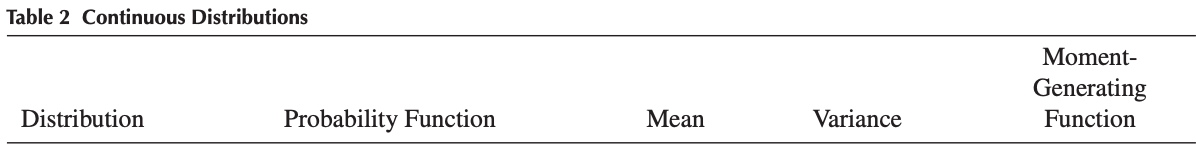
\includegraphics[scale=0.4]{Images/names.png}
    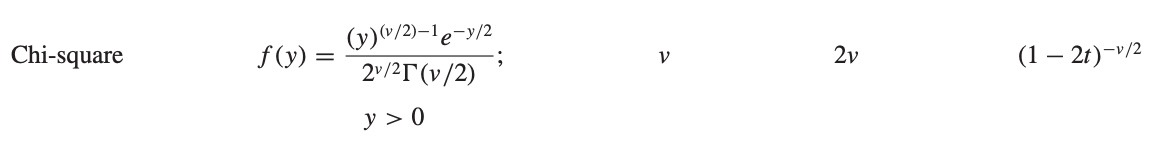
\includegraphics[scale=0.4]{Images/Chi.png}
\end{center}
La demostración del caso general es la siguiente: 
\begin{align}
    m_U(t) &= E\left(\exp\left(tU\right)\right)\\
           &= \int_{-\infty}^\infty \exp\left(tU\right)\cdot f(U)\ d U &\text{Definición 5.9}\\
           &= \int_{-\infty}^\infty \exp\left(tU\right)\cdot \frac{(U)^{(v/2)-1}\exp\left (-U/2\right)}{2^{v/2}\Gamma(v/2)}\ d U\\
           &= \frac{1}{2^{v/2}\Gamma(v/2)}\int_{0}^\infty \exp\left(tU-U/2\right)\cdot (U)^{(v/2)-1}\ d U\\
           &= \frac{1}{2^{v/2}\Gamma(v/2)}\int_{0}^\infty \exp\left(-U(1/2-t)\right)\cdot (U)^{(v/2)-1}\ d U
           \intertext{Se propone $y=U(\frac{1}{2}-t)$:}
           &= \frac{1}{2^{v/2}\Gamma(v/2)}\int_{0}^\infty \exp\left(-y\right)\cdot \left(\frac{2y}{1-2t}\right)^{(v/2)-1}\cdot \frac{2}{1-2t}\ d U\\
           &= \frac{1}{2^{v/2}\Gamma(v/2)}\int_{0}^\infty \exp\left(-y\right)\cdot \left(\frac{2y}{1-2t}\right)^{(v/2)}\cdot \ d U\\
           &= \frac{1}{2^{v/2}\Gamma(v/2)}\cdot \left(\frac{2}{1-2t}\right)^{(v/2)}\int_{0}^\infty \exp\left(-y\right)\cdot \left(y\right)^{(v/2)}\ d U\\
           &= \frac{1}{2^{v/2}\Gamma(v/2)}\cdot \left(\frac{2}{1-2t}\right)^{(v/2)} \Gamma (\frac{v}{2})\\
           &= \frac{1}{2^{v/2}}\cdot \left(\frac{2}{1-2t}\right)^{(v/2)}\\
           &= \left(\frac{1}{1-2t}\right)^{(v/2)}\\
           &= \left(1-2t\right)^{-v/2}
\intertext{Finalmente, podemos calcular:}
m_W(t) &= m_{X_1}(t)\times m_{X_2}(t)\\
(1-2t)^{-v/2} &= m_{X_1}(t)\times (1-2t)^{-1/2}\\
\intertext{Despejando para $m_{X_1}(t)$:}
m_{X_1}(T) &= (1-2t)^{-(n-1)/2}
\end{align}
Por lo tanto, se tiene que por medio de la función generado de momento de $X_1=\frac{\sum_{i=1}^n(Y_i-\overline{Y})^2}{\sigma^2}$ tiene una distribución $\chi^2$ con $n-1$ gl.
\end{proof}

\end{enumerate}(Valor 2 puntos)






%---------------------------
\bibliographystyle{apalike}
\bibliography{sample.bib}

\end{document}